\section{Relaciones del lenguaje NDTI}
\label{sec:relaciones_ndti}

\noindent
Las relaciones definidas en el lenguaje NDTI permiten establecer vínculos semánticos entre los distintos elementos del modelo. Estas se clasifican en relaciones de tipo estructural y conductual, dependiendo de si representan dependencias estáticas o interacciones dinámicas dentro del sistema.

\begin{longtable}{|
>{\centering\arraybackslash}m{1.5cm}|
>{\centering\arraybackslash}m{2.8cm}|
>{\centering\arraybackslash}m{2.2cm}|
>{\raggedright\arraybackslash}m{4cm}|
>{\raggedright\arraybackslash}m{4cm}|}
\caption{Relaciones del lenguaje NDTI} \label{tab:relaciones_ndti_formal} \\

\hline
\textbf{Ícono} & \textbf{Relación} & \textbf{Tipo} & \textbf{Definición semántica} & \textbf{Regla de uso} \\
\hline
\endfirsthead

\hline
\textbf{Ícono} & \textbf{Relación} & \textbf{Tipo} & \textbf{Definición semántica} & \textbf{Regla de uso} \\
\hline
\endhead

\hline
\endfoot

\hline
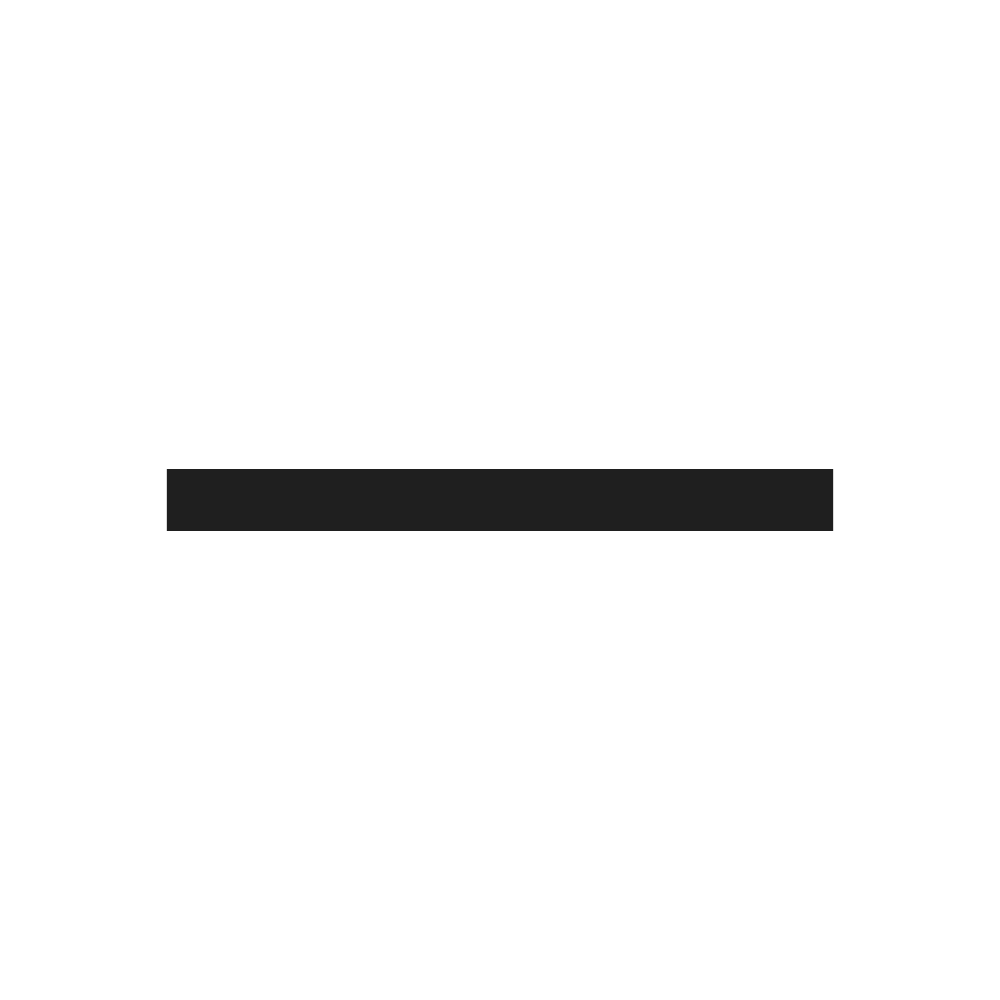
\includegraphics[width=1.1cm]{tablas-images/relaciones/ndti_assoc.png}
& R-01 Asociación
& Estructural
& Establece una relación genérica entre dos elementos sin implicar una semántica específica más allá de su vinculación.
& Se emplea únicamente cuando no es posible o necesario definir una relación más específica entre los elementos. \\
\hline

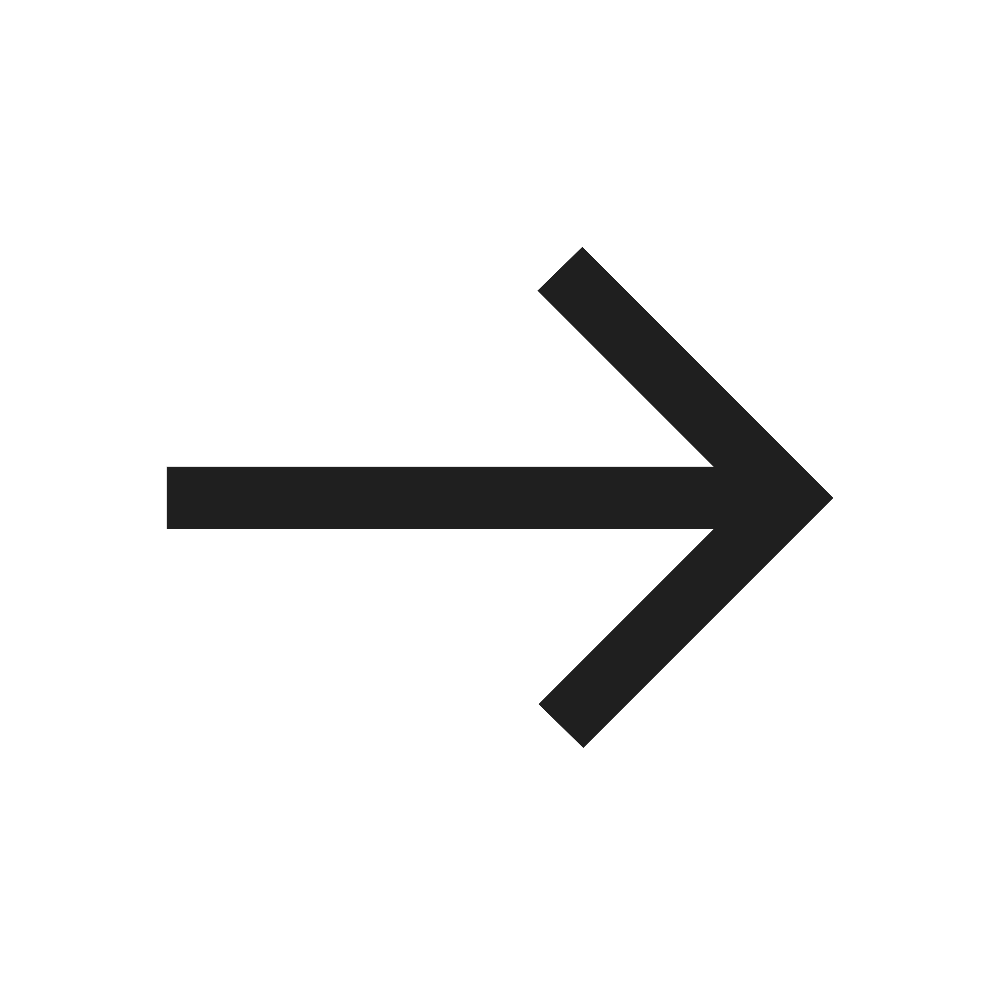
\includegraphics[width=1.1cm]{tablas-images/relaciones/ndti_flow.png}
& R-02 Flujo
& Conductual
& Representa la transferencia de información, datos o control entre elementos dentro de un proceso o interacción.
& Debe utilizarse exclusivamente entre elementos de comportamiento, como procesos, funciones o eventos. \\
\hline


\includegraphics[width=1.1cm]{tablas-images/relaciones/ndti_dependency.png}
& R-03 Dependencia
& Estructural
& Indica que un elemento requiere de otro para su funcionamiento, sin implicar una relación de contención.
& Se utiliza cuando un elemento depende funcionalmente de otro, sin que exista una relación jerárquica o de composición. \\
\hline


\includegraphics[width=1.1cm]{tablas-images/relaciones/ndti_realization.png}
& R-04 Realización
& Estructural
& Señala que un elemento implementa, materializa o concreta a otro en un nivel más específico.
& Debe emplearse para relacionar elementos abstractos con sus implementaciones, típicamente entre distintas capas del modelo. \\
\hline

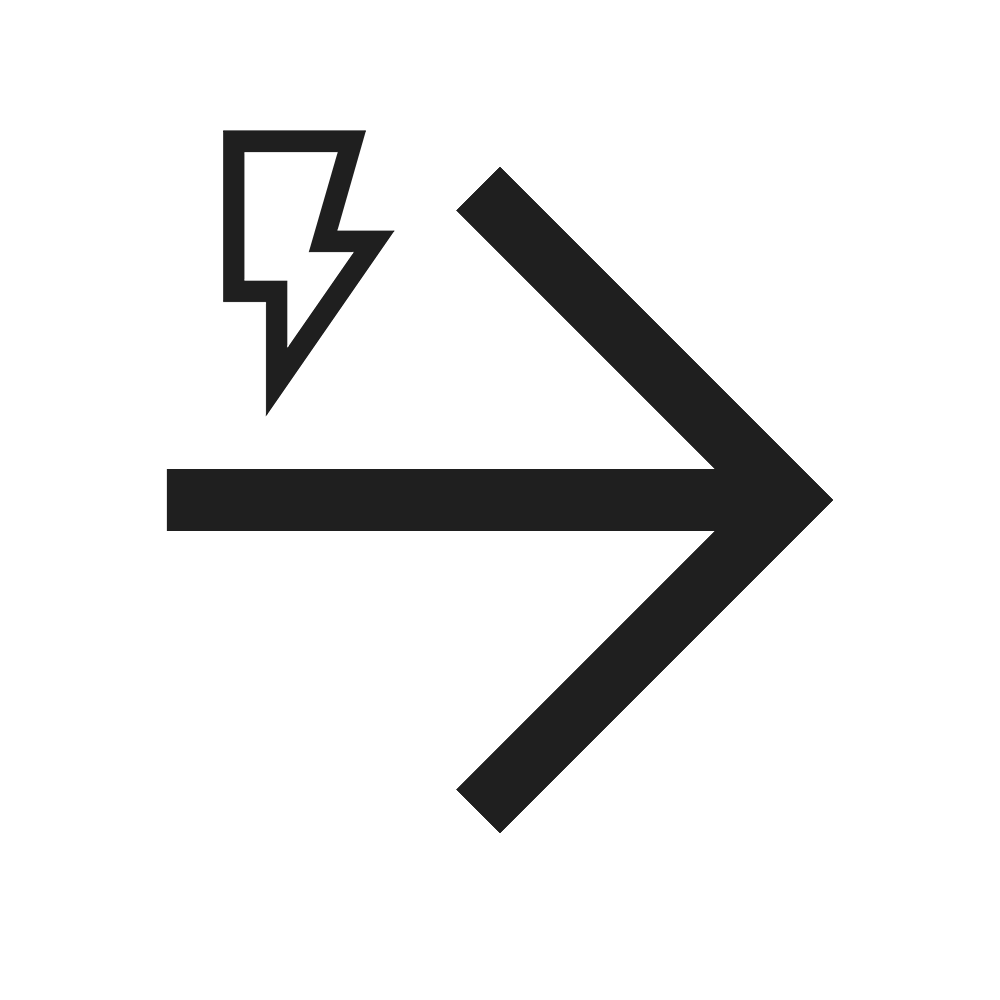
\includegraphics[width=1.1cm]{tablas-images/relaciones/ndti_trigger.png}
& R-05 Trigger
& Conductual
& Representa una relación causal en la que un elemento inicia o activa el comportamiento de otro.
& Se utiliza principalmente para modelar la activación de procesos o funciones a partir de eventos. \\
\hline


\includegraphics[width=1.1cm]{tablas-images/relaciones/ndti_generalization.png}
& R-06 Especialización
& Estructural
& Define una relación jerárquica en la cual un elemento hereda características de otro más general.
& Debe utilizarse para representar estructuras jerárquicas o taxonomías entre elementos del mismo tipo conceptual. \\
\hline


\includegraphics[width=1.1cm]{tablas-images/relaciones/ndti_comm.png}
& R-07 Comunicación
& Conductual
& Representa el intercambio de información entre dos o más elementos de forma bidireccional o colaborativa.
& Se utiliza en interacciones entre actores, componentes o procesos que intercambian información de manera continua. \\
\hline

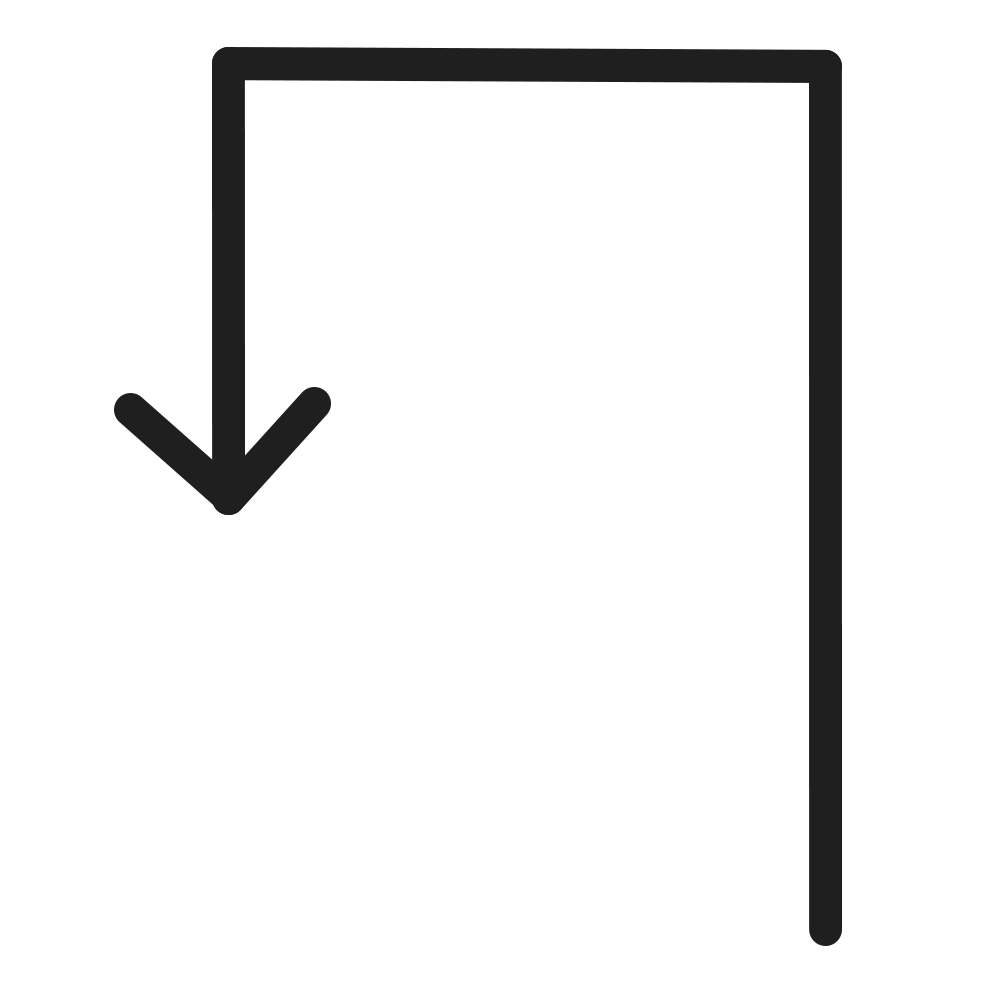
\includegraphics[width=1.1cm]{tablas-images/archi/business/ndti_loop.png}
& R-08 Bucle
& Conductual
& Representa la repetición de una o varias actividades dentro de un proceso hasta que se cumpla una condición determinada.
& Se utiliza exclusivamente dentro de procesos para modelar comportamientos iterativos. \\
\hline


\includegraphics[width=1.1cm]{tablas-images/archi/business/ndti_parallel.png}
& R-09 Paralelización
& Conductual
& Indica la ejecución concurrente de múltiples actividades dentro de un proceso.
& Se emplea para representar bifurcaciones o sincronizaciones de flujos paralelos en procesos. \\
\hline

\end{longtable}

\subsection{Clasificación de relaciones}

\noindent
Las relaciones del lenguaje NDTI se clasifican en:

\begin{itemize}
\item \textbf{Relaciones estructurales:} describen dependencias estáticas entre elementos.
\item \textbf{Relaciones conductuales:} representan interacciones dinámicas y flujos de ejecución.
\end{itemize}

\subsection{Restricciones generales}

\begin{itemize}
\item Las relaciones conductuales solo pueden establecerse entre elementos de comportamiento.
\item Las relaciones estructurales deben mantener coherencia semántica entre los elementos conectados.
\item La relación de especialización solo puede aplicarse entre elementos del mismo tipo conceptual.
\end{itemize}